\chapter{Aplicação de técnicas de usabilidade em desenvolvimento de software empírico }

	Esse capítulo introduz os modelos de ciclos de vida existente na engenharia de usabilidade e interação humano computador e informa sobre o que se tem feito para aplicar as técnicas de usabilidade no processo ágil de desenvolvimento de software.

\section {Usabilidade em Software Livre}

	Um dos grandes problemas encontrados em softwares livres é a pouca atenção dada aos aspectos referentes a usabilidade e acessibilidade das aplicações. Acredita-se que um dos principais problemas que contribui para a falta de usabilidade de software livre é sua própria comunidade que apenas enfatiza na criação e, melhoria e teste do código fonte.  

Segundo ~\citeonline{preece2007}, uma das causas da baixa adoção de softwares livres em mercados de larga escala é a baixa qualidade dos estilos de interação implementados nas interfaces dos produtos. Uma grande maioria não se preocupa com bons elementos de interface com usuário (UI). 

Atualmente, algumas comunidades de software livre vêm se atentando as questões de usabilidade como forma de se manter no mercado. Um dos casos que conhecemos foi do Joomla que é um sistema de gerenciamento de conteúdo  que nessas últimas versões investiram em questões de usabilidade, sendo o primeiro CMS a ser 100 por cento responsivo. Foi criada uma frente de desenvolvimento focado na experência do usuário que trouxe melhorias significativas a partir da versão 3.0 do CMS. Logo em seguida o Wordpress, outro sistema de gerenciamento de contéudo investiu em melhorias da interface se atentando aos novos padrões adotados na web.

	Uma grande dificuldade encontrada por parte de usuários com pouca experiência se encontra na instalação de softwares livres o que acaba por desencorajar esses usuários na utilização desses softwares.
	
Entender o perfil do usuário é um dos principais pontos que devem ser levados em consideração pelos desenvolvedores de software em geral. Cada perfil de usuário tem suas particularidades e suas expectativas quanto a utilização do sistema. Quando falamos de usuários com experiência de uso de softwares semelhantes é preciso ter uma maior atenção na usabilidade para que possa ter uma boa aceitação e menor impacto com as mudanças.

De acordo com observações feitas, percebeu-se que algumas pessoas que trabalham com desenvolvimento de software não conhece exatamente o que significa usabilidade.  Muitas acham que usabilidade é apenas ter uma interface bonita e agradável aos olhos dos usuários e esquecem o real significado do termo usabilidade. 

É dito que um sistema tem usabilidade quando o usuário encontra facilmente o que deseja e executa uma tarefa de forma rápida, intuitiva e simples. Um sistema feito apenas para um terminal pode ter uma boa usabilidade.

%---------------------------------------------------------%

\section{Modelos de Ciclo de Vida}

	Exitem 2 grandes abordagens para o desenvolvimento de software: A abordagem tradicional sendo o seu principal método o (RUP - Rational Unified Process) e a abordagem ágil. Nesse trabalho iremos abordar somente os métodos ágeis de desenvolvimento de software que é a base de nosso estudo e como podemos integrar a usabilidade no ciclo de vida de desenvolvimento de software empírico.No capítulo 2 definimos sobre o que são os métodos empíricos de desenvolvimento de software.

	Para que possamos conhecer o processo completo de desenvolvimento é importante considerar as como as atividades se relacionam. Entender que atividades estão envolvidas no design de interação é o primeiro passo para estar apto à faze-lo.

	O termo modelo de ciclo de vida é utilizado para representar um modelo que capta um conjunto de atividades e a maneira como elas se relacionam ~\cite{preece2005}.Existe alguns modelos de processo de engenharia de usabilidade:

\begin{itemize}
\item Modelo Estrela
\item Ciclo de vida de Engenharia de Usabilidade
\item Projeto Centrado no Usuário da Norma ISO/IEC 13407
\end{itemize}

\subsection{Modelo Estrela}

	Proposto em 1989 por Hartson e Hix, o modelo de ciclo de vida estrela derivou do trabalho empírico de entender como os designers lidavam com os problemas de design em IHC.Eles observaram dois diferentes modelos de trabalho: analítico e o sintético. O primeiro parte-se da visão do sistema para a visão do usuário, já o segundo da visão do usuário para a do sistema ~\cite{cybis2010}.

	No modelo estrela não há especificação de ordenamento de atividades. Pode-se ir de uma atividade à outra há qualquer momento, desde que passe primeiramente pela avaliação.Sempre que uma atividade for completada deve-se avaliar o seus resultados.

\begin{figure}[h]
    \centering
    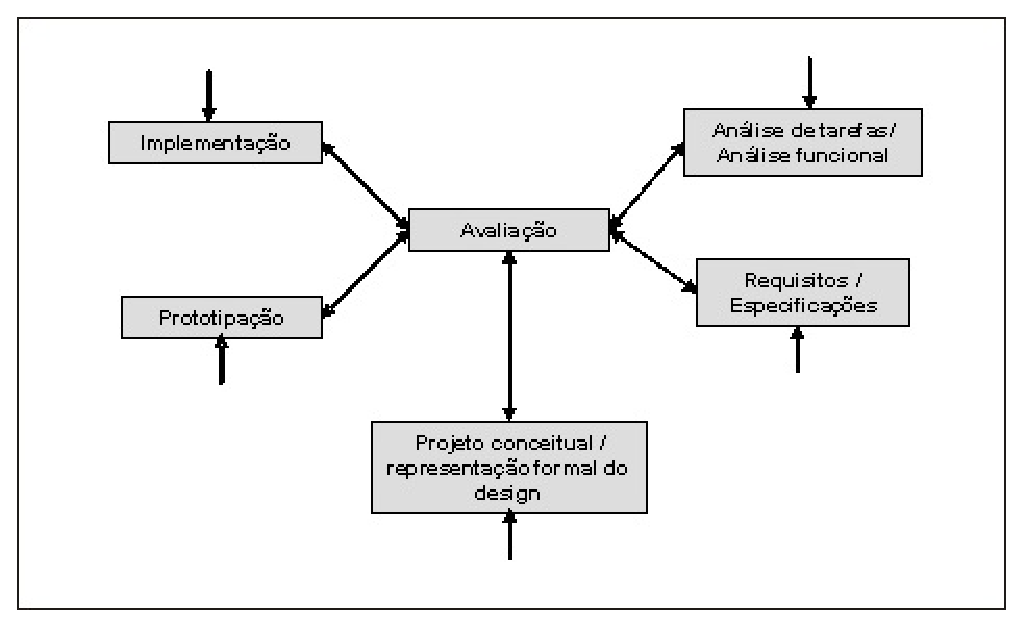
\includegraphics[keepaspectratio=true,scale=0.60]
      {figuras/estrela.eps}
    \caption{Ciclo de Vida Estrela~\cite{preece2005}}
    \label{ciclo_estrela}
\end{figure}

\subsection{O ciclo de vida da Engenharia de Usabilidade - Mayhew}

	O ciclo de vida de engenharia de usabilidade foi proposto por Deborah Mayhew em 1999. A ISO 13407 também propõe um modelo de ciclo de concepção centrado no usuário. Ambos possuem a mesma estrutura e propõem ciclos de atividades de análise, projeto, construção e testes ~\cite{cybis2010}.

	O ciclo proposto por ~\citeonline{mayhew1999} oferece uma visão holística acerca dessa engenharia e uma descrição detalhada de como podemos realizar os testes de usabilidade ~\cite{preece2005}.

	A primeira etapa do ciclo é a análise dos requisitos.Mayhew propõe quatro tipos de atividades de análise de requisitos que são detalhadas abaixo:

\begin{itemize}
\item \textbf{Análise do perfil do usuário:} Os projetistas devem conhecer os atributos pessoais e suas habilidades para cada tipo de usuário identificado. 
	
\item \textbf{Análise do contexto da tarefa:} Os projetistas devem conhecer os objetivos e resultados, a estrutura, duração, custos e etc. de cada tarefa a ser realizada.

\item \textbf{Análise das possibilidades e restrições da plataforma:} Verificar quais são as possibilidades e restrições em termos de equipamentos, sistems operacionais e etc.

\item \textbf{Análise dos princípios gerais para o projeto:} Atividade relacionada à pesquisa e catalogação dos conhecimentos de ergonomia disponível para a concepção da interface no tipo de contexto de uso.

\end{itemize}

%inserir figura de requisitos ?

	Depois da análise dos requisitos é preciso especificar as metas de usabilidade do futuro sistema. A norma ISO 9241:11 orienta como podemos especificar essas metas.

	%falar sobre as medidas de usabilidade geral? fatores de usabilidade ou ter uma seção somente para falar das métricas?

	Na etapa de projetos, testes e implementação, Mayhew propôs que os ciclos devem se repetir de forma a tratar três nivéis de aspectos de uma interface: No primeiro nível sendo a interface definida conceitualmente; no segundo nível refere-se as definições em termos de estilo; e no terceiro nível as interações e componentes relacionados com os contextos das tarefas especiais.A figura mostra o passo a passo da etapa de projetos/testes e implementação.
	A última fase é a de instalação do sistema onde depois que o usuário já estiver acostumado com o sistema ele pode dar um feedback sobre a usabilidade do produto de forma mais fidedigna por já ser um "especialista" da ferramenta como cita a autora. 

%inserir figura.

	Uma das técnicas utilizadas para coletar feedback são os testes de usabilidade no local do trabalho dos usuários ou utilizando métodos de análise como entrevistas, observações, questionários, grupos de discussões. Esses métodos serão detalhados no pŕoximo cápitulo.


\subsection{Design Centrado no usuário - ISO/IEC 13407}

O DCU surgiu da IHC e consiste em uma metodologia de design de software para desenvolvedores e designers. Foi definida pela norma ISO 13407 (Human Centered Design Processes for Interactive Systems) e tem como objetivo definir um processo necessário ao desenvolvimento de produtos fáceis de utilizar na qual deve envolver os usuários no processo de desenvolvimento e na avaliação dos produtos.

Sabemos que a ciência experimental que utiliza-se dos métodos empíricos tradicionais para coletar dados e testar hipóteses sobre o comportamento humano aplicam-se de várias técnicas em nome de pessoas.Essa abordagem é preocupada com os usuários quando as representa mas ela não leva em conta diversos aspectos do usuário real, por não envolvê-los no processo. Não basta fazer para o usuário, é preciso fazer com o usuário ~\cite{eason1995}. 

No Design Centrado no usuário (DCU) diferente dos métodos empíricos tradicionais que tem o usuário apenas como  referência, no DCU o usuário tem que ser o elemento central e é necessário envolvê-lo do início ao fim do projeto.Baseia-se nas necessidades, desejos e limitações das pessoas. Deve-se iniciar com usuários e suas necessidades em vez de começar com a tecnologia (Várias fontes ?). ~\citeonline{travis2013} afirma que "para criar produtos que os usuário amem, é necessário incluir os usuários no processo de criação dos produtos". 

Gould e Lewis estabeleceram alguns princípios para o desenvolvimento centrado no usuário na decada 70 que são utilizados até hoje que são: Foco desde o inicio nos usuários e nas tarefas, medidas empiricas e design interativo.O processo do design centrado no usuário pode ser dividido em 3 fases: análise, desenvolvimento e pós-liberação. 

%	Detalhar o fluxo do DCU

\subsubsection{ISO 13407 e 9241-210}
	
A ISO 13407 define um processo geral para incluir atividades centradas em humano através do ciclo de vida de desenvolvimento sem especificar métodos exatos ~\cite{santos2012}.

A norma é caracterizado por quatro princípios: Ativo envolvimento do usuário; alocação apropriada de funções entre usuários e tecnologia; Testes de solução de design; Design multidisciplinar.Em 2010 essa ISO foi revista e renomeada para a ISO 9241-210.

Existem quatro atividades de Design Centrado no Usuário que devem estar presentes no inicío do projeto:

\begin{itemize}
\item Entender e especificar o contexto de uso;
\item Especificar os requisitos de usuário;
\item Produzir soluções de design;
\item Avaliar o design frente aos requisitos;
\end{itemize}

A ISO 13407 propõe que o envolvimento do usuário seja uma prática frequente em empresas que desenvolvem sistemas interativos.

\begin{figure}[h]
    \centering
    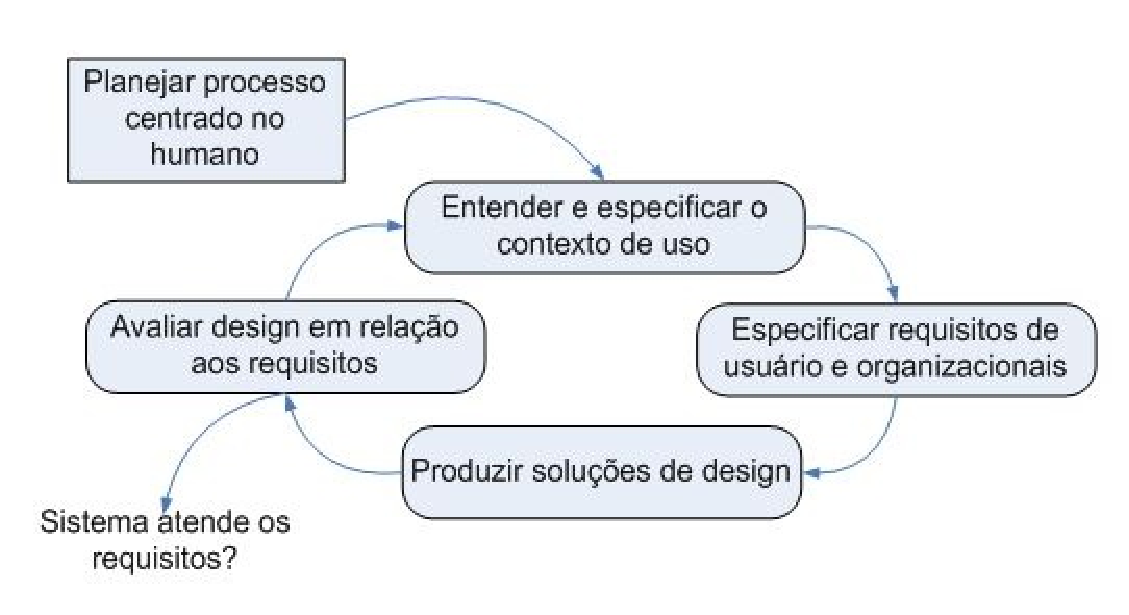
\includegraphics[keepaspectratio=true,scale=0.60]
      {figuras/ciclo_iso13407.eps}
    \caption{Ciclo do Design centrado no humano - Norma ISO 13407~\cite{iso13407}}
    \label{ciclo_iso13407}
\end{figure}


%------------------------------------------------------------------------------%

% Inicio da Seção sobre métodos ágeis e o design centrdo no usuário

\section{Métodos Ágeis e o Design Centrado no usuário}

	Os métodos ágeis é uma abordagem de desenvolvimento que têm como princípio ....%ver como escrever isso
Muitos autores têm defendido a ideia da integração dos aspectos da usabilidade com os métodos ágeis.
	
	Um dos grandes problemas da integração dessas duas metodologias é o fato de que elas utilizam-se de abordagens diferentes sobre como os recursos são alocados e como a defesa da coleta de requisitos e projetos de forma antecipada, mas as abordagens são centradas no usuário.

	Há uma semelhança entre os valores da abordagem ágil e a de IHC proporcionando um quadro favorável à integração minimalista de pŕaticas de IHC em ambientes ágeis.Podemos citar alguns desse valores como por exemplo: (i) ciclos curtos com entregas contínuas e incrementais, que favorecem a aplicação de técnicas de prototipagem; (ii) forte envolvimento do usuário que favorece a aplicação de princípios de projetos participativos e (iii) programação em pares onde em IHC geralmente a avaliação de usabilidade é feita em pares ~\cite{barbosa2008estrategia}. 

	Segundo ~\citeonline{cybis2010} as características da abordagem ágil facilitam na utilização da ergonomia e da usabilidade durante o desenvolvimento de software, mas afirma que os ergonomistas e engenheiros de usabilidade deverão adaptar suas técnicas de análise, modelagem, projeto e teste adotando-se os preceitos do manifesto ágil.
	
	As adaptações são realmente necessárias, principalmente na questão da granularidade da pesquisa, no tempo gasto com ela e na maneira de relatar as descobertas de usabilidade ~\cite{santos2012}.

\subsection{DCU Ágil}


        Pode ser definido o DCU ágil como a prática de design centrado no usuário quando conduzida dentro de uma metodologia ou filosofia de desenvovlimento ágil de software.~\cite{santos2012}

	O ciclo de DCU ágil foi proposto por ~\citeonline{sy2007adapting} e integra tantos as atividades de DCU como as de desenvolvimento em um único ciclo, trabalhando nas mesmas características e garantindo que as investigações de usabilidade serão tratadas durante a interação.


%Figura do ciclo do DCU ágil

	
	O grande desafio do DCU ágil é de encontrar a melhor maneira de realizar as atividades de pesquisa do usuário, design de versões que atendem as necessidades dos usuário, construção de versões interativas e realização de testes de usabilidade, dentro de um ambiente de desenvolvimento com métodos ágeis, tendo a participação dos usuários tipicos em todas as atividades ~\cite{santos2012}.% (Copia da Ana Paula) - Verificar como reescrever.
	
        A modelagem e projeto de interfaces devem ser orientados a padrões de projeto e as avaliações de ergonomia, testes de usabilidade e especificações de revisões de interface devem ser realizados rapidamente ~\cite{cybis2010}.
	
	Pesquisas relatam que praticantes de UX que passaram a trabalhar em ambientes ágeis não querem mais retornar ao método antigo de desenvolvimento baseado no modelo cascata. Em média, essas equipes levam de 6 a 12 meses para se adptar ao novo ambiente ~\cite{santos2012}.

	O termo experiência do usuário é utilizado na comunidade ágil para qualquer atividade relacionada com a pesquisa do usuário, DCU, usabilidade, design de interfaces.A utilização do termo não indica que eles realizam todas as atividades de UX ~\cite{santos2012}.

	Segundo ~\citeonline{dickinson2010} a chave para a integração de DCU com métodos ágeis é assegurar que os resultados da pesquisa de usuário são comunicados e entendidos de forma eficaz dentro de uma equipe ágil.


\subsection {DCU e XP}

	Foram encontrados alguns estudos que descrevem a integração do IHC com as práticas de Programação Extrema (XP). Segundo ~\citeonline{mcinerney2005ucd} métodos ágeis e design centrado no usuário possuem uma cultura distinta mas eles mostraram que é possivel unir essas duas abordagens. Em seu artigo ....

	O processo de usabilidade ágil é integrar os instrumentos de IHC dentro dos processos clássico de XP. ~\citeonline{wolkerstorfer2008probing} usam o dcu ágil desde 2007 e que até hoje não houve nenhum problema entre as culturas e que tanto os especialistas de usabilidade quanto os desenvolvedores estão bem integrados.Pode-se encontrar vantagens na combinação das duas abordagens. 

	Em 2008 foi proposto uma metodologia revisional institulada XPlus que insere as técnicas de design e de usabilidade em determinadas fases do ciclo de desenvolvimento de software.O XPlus agrega algumas práticas de User Experience às práticas tradicionais de XP. A figura mostra uma visão geral do processo de desenvolvimento de software de XPlus.

	Essa metodologia considera a interface um dos aspectos mais importantes de um software.Ela envolve as novas pŕaticas de UX no processo natural de XP.

	O papel de designer de interação não é reconhecido no núcleo eXtreme Programming (XP) da equipe e o XP não tem nenhum processo explícito para lidar com o design de interação.Em seu estudo ~\citeonline{ferreira2007interaction} relatam como as equipes combinaram as atividades de design de interação com o XP. 

	A natureza iterativa de desenvolvimento XP necessário que os designers de interação tem envolvimento contínuo com o desenvolvimento do produto influenciou a natureza da relação entre os designers de interação e os desenvolvedores.

	 
%Acrecentar informações da dissertação que achou sobre XP.


\subsection{AgilUS}

	Outra metodologia encontrada foi a de AgilUS que é um método de desenvolvimento ágil que baseia-se no conceito de usabilidade e na necessidade de desenvolver software usável. Essa metodologia foi resultado de uma das linhas de investigação desenvolvida pelo Centro de Engenharia de Software da Universidade Central da Venezuela.

	O objetivo do método AgilUS é proporcionar um conjunto de atividades organizadas para construir a usabilidade de design de interface do usuário durante o desenvolvimento do software.


\section{Princípios ágeis aplicados ao DCU}

	Alguns princípios e boas práticas de métodos ágeis foram levantadas para a aplicação no design de sistemas centrado no usuário. (escrever algo)

\begin{enumerate}

\item Coompreender e Identificar as necessidades reais dos usuários

	O Objetivo dessa etapa é conhecer o usuário alvo. Deve-se projetar ferramentas que irão dar suporte aos objetivos e atividades das pessoas.

	Algumas técnicas são utilizadas para identificar as necessidades dos usuários como a observação natural que serve para responder a questão do tipo:o que e como as pessoas fazem? E as entrevistas que responde o que as pessoas pensam e dizem.Os resultados da pesquisa devem ser comunicados para a equipe.

\item Focar na Essência

	 O foco na essência ajuda a desenvolver soluções que atendem às reais necessidades dos usuários diminuindo os riscos de desenvolvimento de funcionalidades com pouco ou nenhum uso.

	A ideia desse príncipio é que deve-se começar a desenvolver apenas pelo que é essencial, começando pela menor unidade de um sistem sem perder a visão de um todo.

\item Iterar mais rápido

	É importante colocar o produto nas mãos dos usuários para se ter um feedback o mais cedo possível.Quando a iteração é feita de forma rápida e começando cedo podemos identificar os problemas com antecedência o que diminui o tempo com retrabalho e evita que o produto não atenda aos usuários.
	

\item Criar designs alternativos

	Rettig em 1994 disse que "para ter uma boa idéia é preciso que se tenha várias". A ideia do autor da frase é que devemos pensar e criar várias soluções para um mesmo problema afim de que possa ter mais possibilidades de escolha. 

	Simular diferentes alternativas de desenho utilizando diferentes técnicas de prototipação desde as fases iniciais de desenvolvimento.

\item Prototipar em baixa resolução

	Os protótipos de baixa resolução permite visualizar uma solução de forma mais rápida e concreta economizando tempo de design e desenvolvimento. Esses prótotipos ajuda a comunicar e entender idéias e serve para validar uma solução.Eles são úteis pois tendem a ser simples, baratos e de rápida produção.

	Um exemplo de prótotipo de baixa fidelidade são os storyboard que será detalhado no pŕoximo cápitulo. 

	A prototipação aumenta a comunicação entre a equipe de desenvolvimento e os usuários finais, funcionando como uma alternativa "barata" para explorar alternativas de desenho.
	
\item Menos documentação, mais comunicação

	É essencial que tenha uma boa comunicação em todo o processo entre os desenvolvedores, designs e stakeholders envolvidos no projeto.

\item Pesquisa e design em paralelo ao desenvolvimento


\item Testes de usabilidades ágeis

	Os testes de usabilidade devem ser feitos em todos os ciclos do projeto. Recomenda-se que os testes sejam feitos mais vezes e que seja menos formal como são feitos atualmente. Os resultados encontrados nos testes deve ser comunicado à equipe para que possa corrigir os erros  graves rapidamente.

	No próximo capítulo detalharemos como funciona um teste de usabilidade, os tipos existentes e as práticas identicadas pela comunidade de arquitetura da informação e áreas correlatas.

\item O fim não é o lançamento

	No fim de cada ciclo lança-se o mínimo adequado às necessidades reais dos usuários. Ao observar o uso real identificamos que existem novas formas para usar a ferramenta e podemos propor novas melhorias para o sistema. 
	
\end{enumerate}



\section{Teste da Usabilidade vs.Teste de Aceitação do Usuário (UAT)}

	Muitas pessoas acreditam que os testes de usabilidade acontece apenas perto do final do desenvolvimento ou do inicio da distribuição quando se tem uma versão em funcionamento. Também essa confusão se dar por conta dos testes de aceitação que são feitas de forma tardia. 

	Teste de Usabilidade e Teste de Aceitação do usuário muitas vezes são confundidos.O UAT pode trazer as questões de usabilidade, mas não é o único método para ser utilizado em um projeto. Por ser feito tardiamente as mudanças baseadas em UAT são muito mais caras. Já os testes de usabilidade foram projetados para oferecer informações verdadeiras de desempenho desde o início do processo.  
	
	O principal objetivo do teste de aceitação do usuário é servir como uma verificação final de a aplicação atendeu aos requisitos funcionais estabelecidos pelo cliente. 



